\section{Results}

\subsection{CPU Results (Apple M1 Pro)}

\subsubsection{Deposit-Kernel Runtime}
Figure~\ref{fig:runtime} shows deposit-kernel runtime versus $N_p$ at $128^2$ resolution with SoA layout and sorted particles.
At $N_p=10^5$, NGP completes in 1.99\,ms, CIC in 0.59\,ms, TSC in 0.90\,ms, and Esirkepov in 4.33\,ms.
At $N_p=10^6$, Esirkepov reaches 52.4\,ms compared with 6.81\,ms for CIC.
CIC is the fastest scheme at moderate $N_p$; Esirkepov is roughly $7\times$ slower than CIC after sparse trajectory optimization.

\begin{figure}[t]
    \centering
    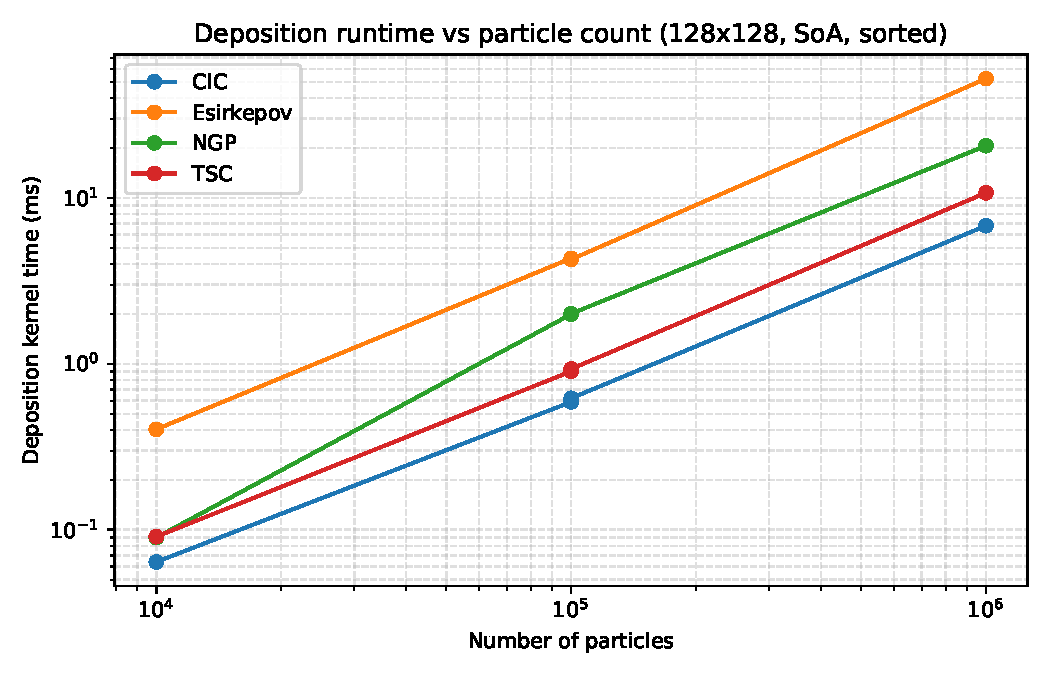
\includegraphics[width=\linewidth]{figures/fig1_runtime_vs_particles.pdf}
    \caption{Deposit-kernel runtime vs.\ particle count ($128\times128$ grid, SoA, sorted, M1 Pro).}
    \label{fig:runtime}
\end{figure}

\subsubsection{Memory Bandwidth}
Figure~\ref{fig:bandwidth} reports effective bandwidth versus grid size at $N_p=10^5$.
CIC achieves approximately 12.4\,GB/s on the $128^2$ grid; NGP is lower ($\sim$2.5\,GB/s) because it performs fewer writes per particle.
TSC bandwidth is comparable to CIC ($\sim$12.6\,GB/s) despite nine writes, reflecting similar memory traffic at this particle density.
Esirkepov reports under 1.7\,GB/s because trajectory weight computation adds per-particle overhead beyond scatter bandwidth.

\begin{figure}[t]
    \centering
    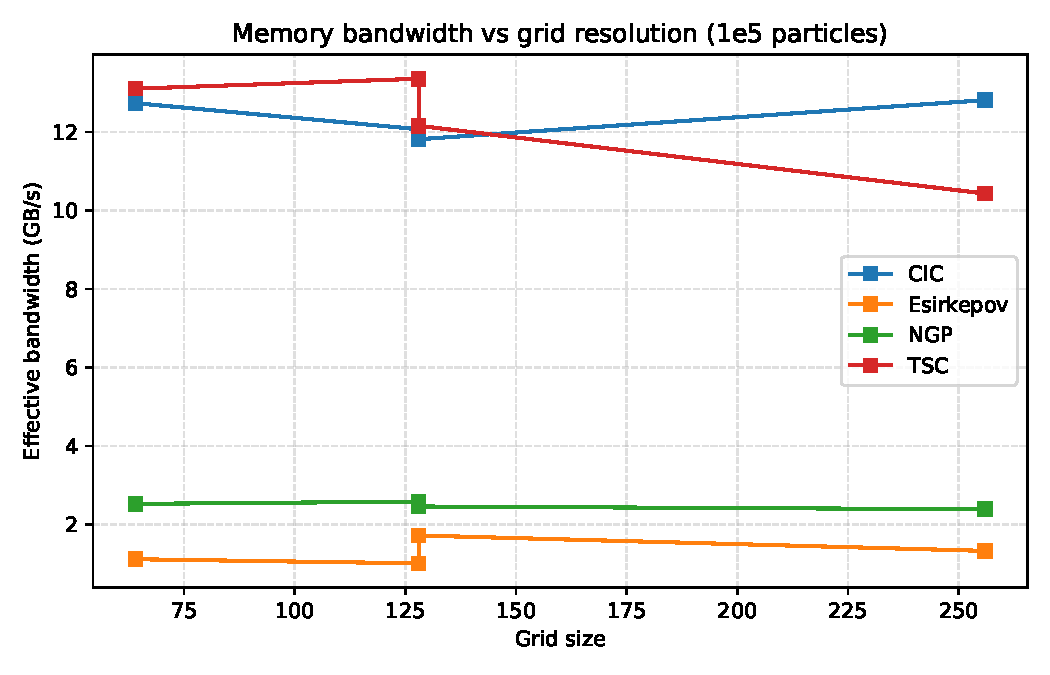
\includegraphics[width=\linewidth]{figures/fig2_bandwidth_vs_grid.pdf}
    \caption{Effective memory bandwidth vs.\ grid size ($10^5$ particles, M1 Pro).}
    \label{fig:bandwidth}
\end{figure}

\subsubsection{Charge Conservation and Energy Drift}
Figure~\ref{fig:charge} and Table~\ref{tab:summary} report $\epsilon_Q$ after a single deposition pass.
NGP achieves zero normalized error in the static test because each particle deposits its full charge to one node.
CIC and TSC remain at machine precision ($\lesssim 10^{-17}$).
Esirkepov shows higher single-step error ($\sim 10^{-3}$) in static microbenchmarks with finite $\Delta t$ on a charge-neutral Maxwellian, but maintains low drift in full 500-step PIC cycles after the corrected deposit-before-push ordering.

\begin{figure}[t]
    \centering
    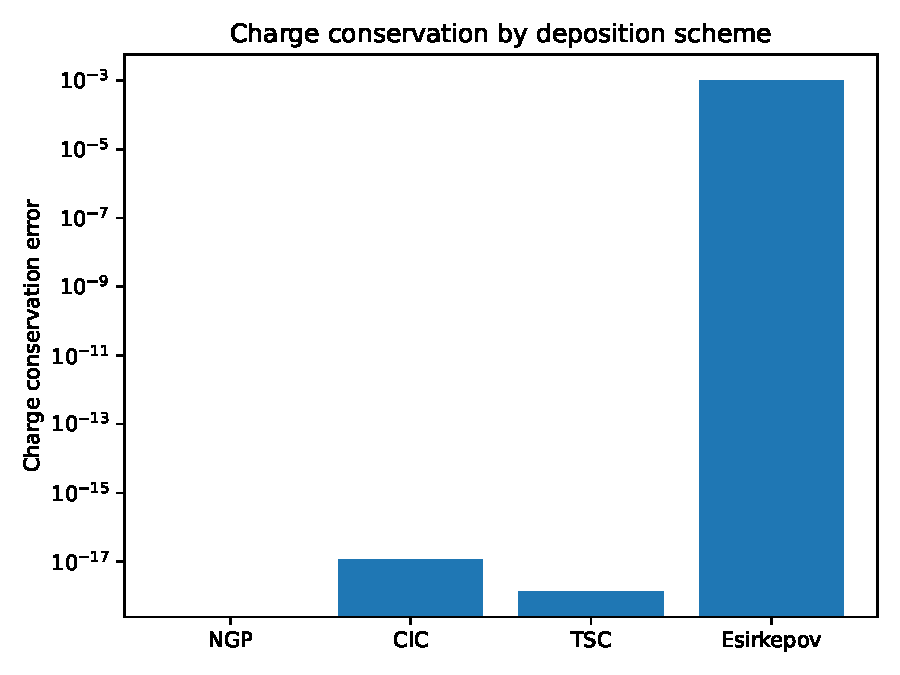
\includegraphics[width=\linewidth]{figures/fig3_charge_error.pdf}
    \caption{Charge conservation error by deposition scheme (M1 Pro).}
    \label{fig:charge}
\end{figure}

Figure~\ref{fig:energy} shows relative total-energy drift after 500 leapfrog steps.
NGP exhibits the largest drift ($\sim -6.6\times 10^{-6}$), consistent with its high grid noise.
CIC and TSC remain at $\sim 10^{-5}$.
Esirkepov drift improves to $\sim -3.0\times 10^{-3}$ with corrected timestep ordering, remaining larger than CIC due to the interaction of trajectory deposition with the leapfrog field solve.

\begin{figure}[t]
    \centering
    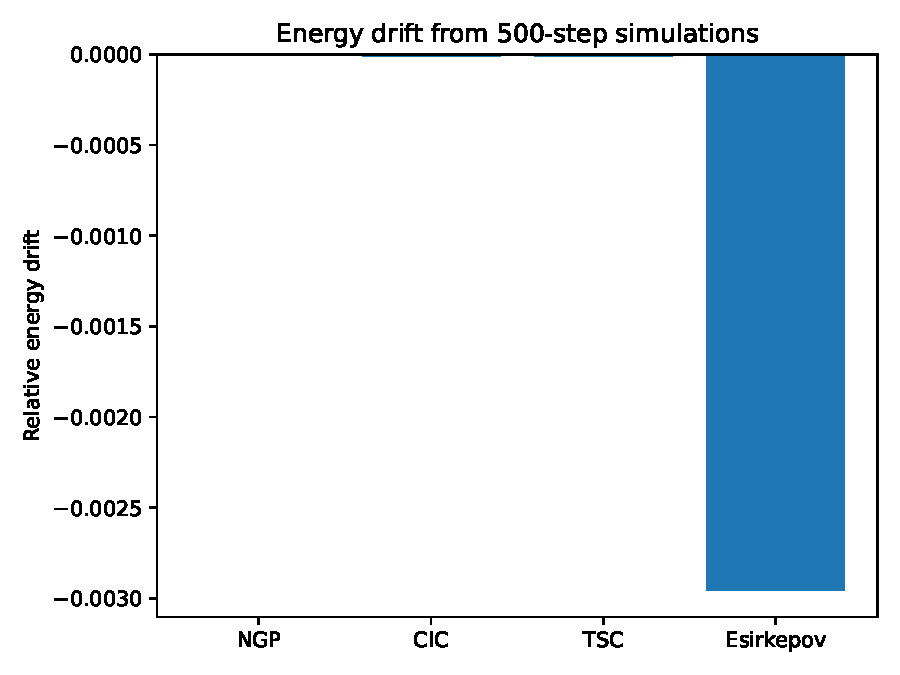
\includegraphics[width=\linewidth]{figures/fig4_energy_drift.pdf}
    \caption{Relative energy drift from 500-step simulations (M1 Pro).}
    \label{fig:energy}
\end{figure}

\subsubsection{OpenMP Strong Scaling}
Figure~\ref{fig:scaling} shows strong scaling for CIC with SoA layout and no sorting.
Deposit time drops from 0.77\,ms at $T{=}1$ to 0.38\,ms at $T{=}2$, 0.44\,ms at $T{=}4$, and 0.18\,ms at $T{=}8$, yielding a $4.4\times$ speedup.
Throughput gains flatten beyond two threads because privatized-grid merge and memory traffic dominate.

\begin{figure}[t]
    \centering
    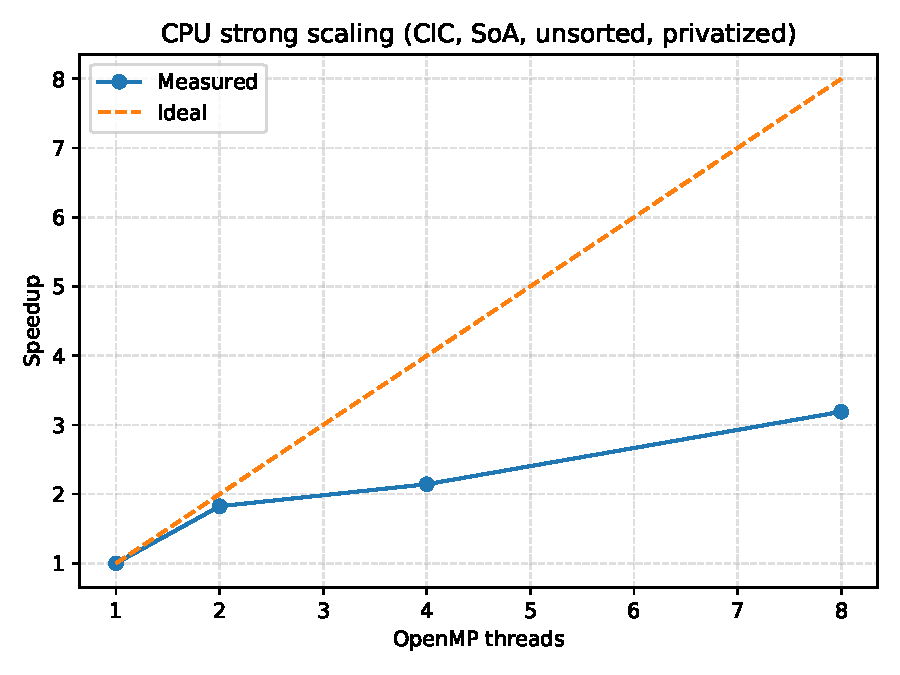
\includegraphics[width=\linewidth]{figures/fig5_cpu_scaling.pdf}
    \caption{OpenMP strong scaling for CIC deposition with privatized buffers (M1 Pro).}
    \label{fig:scaling}
\end{figure}

\subsubsection{Spectral Noise and Layout Overhead}
Figure~\ref{fig:noise} quantifies the high-$k$ power fraction of deposited $\rho$ for a uniform Maxwellian.
NGP noise ratio is 0.61, CIC 0.39, TSC 0.26, and Esirkepov 0.39 in the static deposit test.
TSC delivers the smoothest density field; NGP injects the most short-wavelength content.

\begin{figure}[t]
    \centering
    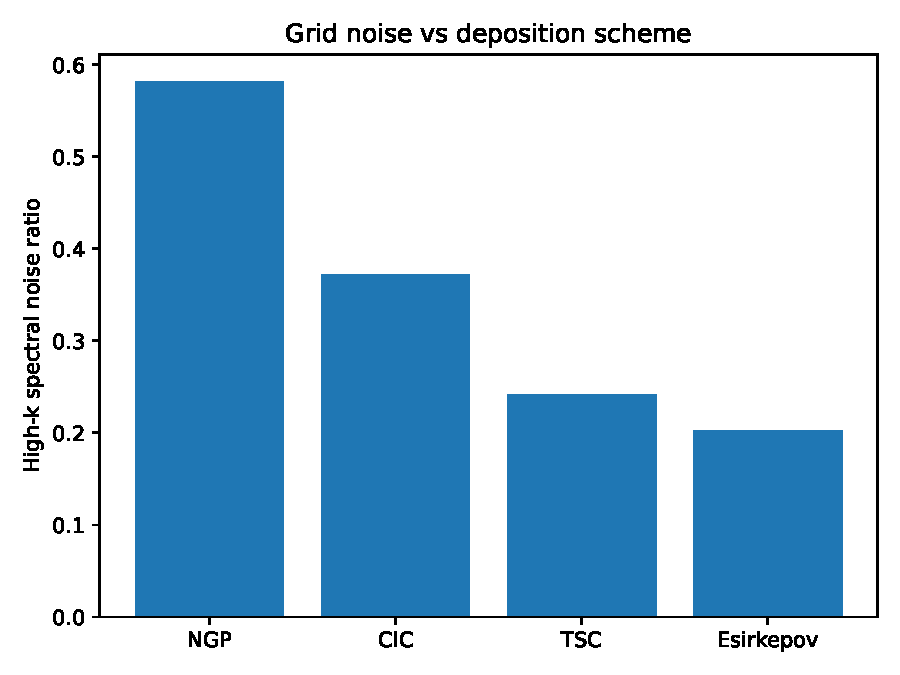
\includegraphics[width=\linewidth]{figures/fig6_spectral_noise.pdf}
    \caption{High-$k$ spectral noise ratio of deposited charge density (M1 Pro).}
    \label{fig:noise}
\end{figure}

Figure~\ref{fig:sort} decomposes total deposition time into sort and deposit components for CIC with SoA layout.
At $N_p=10^5$, sorting costs 2.3\,ms while the deposit kernel takes 0.59\,ms.
SoA and AoS achieve comparable deposit-kernel throughput; SoA sorting is more expensive because reordering requires a gather pass over separate attribute arrays.

\begin{figure}[t]
    \centering
    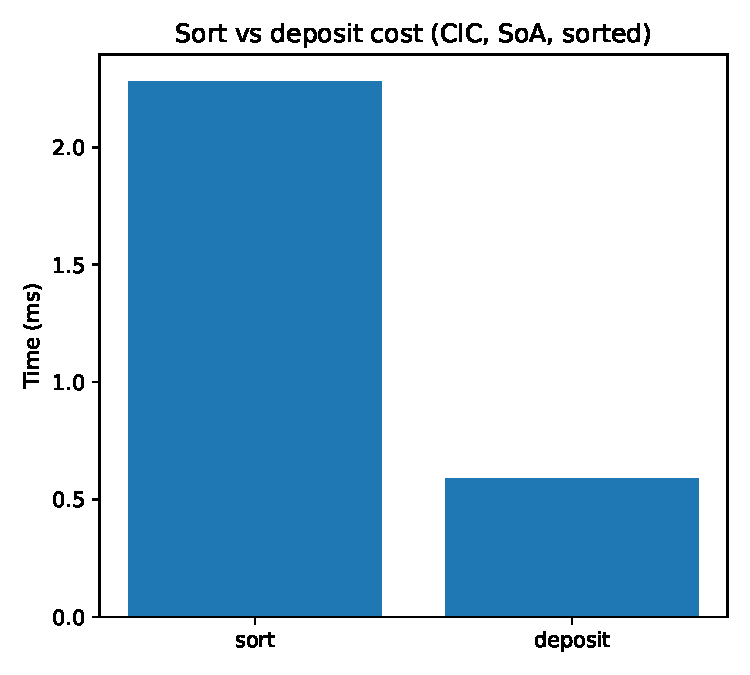
\includegraphics[width=\linewidth]{figures/fig7_layout_sort.pdf}
    \caption{Sort vs.\ deposit time for CIC with SoA layout (M1 Pro).}
    \label{fig:sort}
\end{figure}

Table~\ref{tab:summary} summarizes representative CPU results.
\begin{table}[t]
\centering
\small
\caption{Representative CPU deposition results ($N_p=10^5$, $128^2$ grid, SoA, sorted).}
\label{tab:summary}
\begin{tabular}{lrrrr}
\toprule
Scheme & Sort & Deposit & Thrpt. & $\epsilon_Q$ \\
 & (ms) & (ms) & ($10^8$ p/s) & \\
\midrule
NGP & 2.267 & 1.910 $\pm$ 0.043 & 0.52 & 0.00e+00 \\
CIC & 2.263 & 0.607 $\pm$ 0.061 & 1.65 & 1.16e-17 \\
TSC & 2.421 & 0.848 $\pm$ 0.003 & 1.18 & 1.36e-18 \\
Esirkepov & 2.617 & 7.263 $\pm$ 1.598 & 0.14 & 1.03e-03 \\
\bottomrule
\end{tabular}
\end{table}


\subsubsection{Long-Run Conservation Study}
Figure~\ref{fig:conservation} reports a 2000-step full-PIC conservation study at $N_p=10^4$ on a $64^2$ grid.
CIC and TSC maintain charge error at machine precision with final energy drift below $2\times 10^{-5}$.
NGP preserves charge exactly but shows larger energy drift ($\sim 4\times 10^{-5}$).
Esirkepov exhibits the largest energy drift ($\sim 6\times 10^{-5}$) and occasional charge-error spikes from trajectory crossings, consistent with its higher single-step microbenchmark error.

\begin{figure}[t]
    \centering
    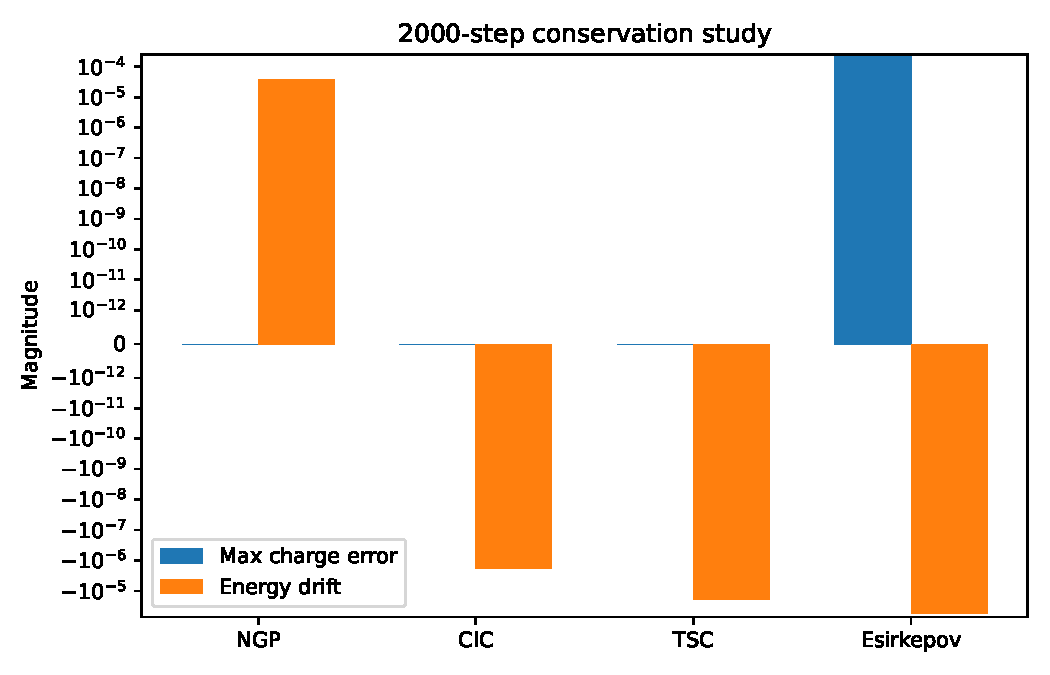
\includegraphics[width=\linewidth]{figures/fig12_conservation_study.pdf}
    \caption{2000-step conservation study: max charge error and final energy drift per scheme.}
    \label{fig:conservation}
\end{figure}

\subsection{GPU Results (Tesla T4, Same Host)}

Figure~\ref{fig:gpu_runtime} compares single-threaded T4-host CPU and atomic GPU deposition at $128^2$ resolution.
At $N_p=10^5$, CIC drops from 4.24\,ms (CPU) to 0.81\,ms (GPU atomics), a $5.3\times$ speedup; TSC achieves $6.3\times$ and NGP $4.4\times$.
At $N_p=10^6$, CIC speedup reaches $7.3\times$ (43.98\,ms $\rightarrow$ 6.07\,ms).
GPU throughput scales more favorably with $N_p$ than the single-core CPU times measured on the T4 host, where PCIe transfer and kernel-launch overhead matter at small particle counts.
Table~\ref{tab:gpu_priv} shows that multi-block privatized CIC achieves machine-precision charge conservation but is $5$--$6\times$ slower than atomics at $128^2$ because each spatial tile scans all particles.

\begin{figure}[t]
    \centering
    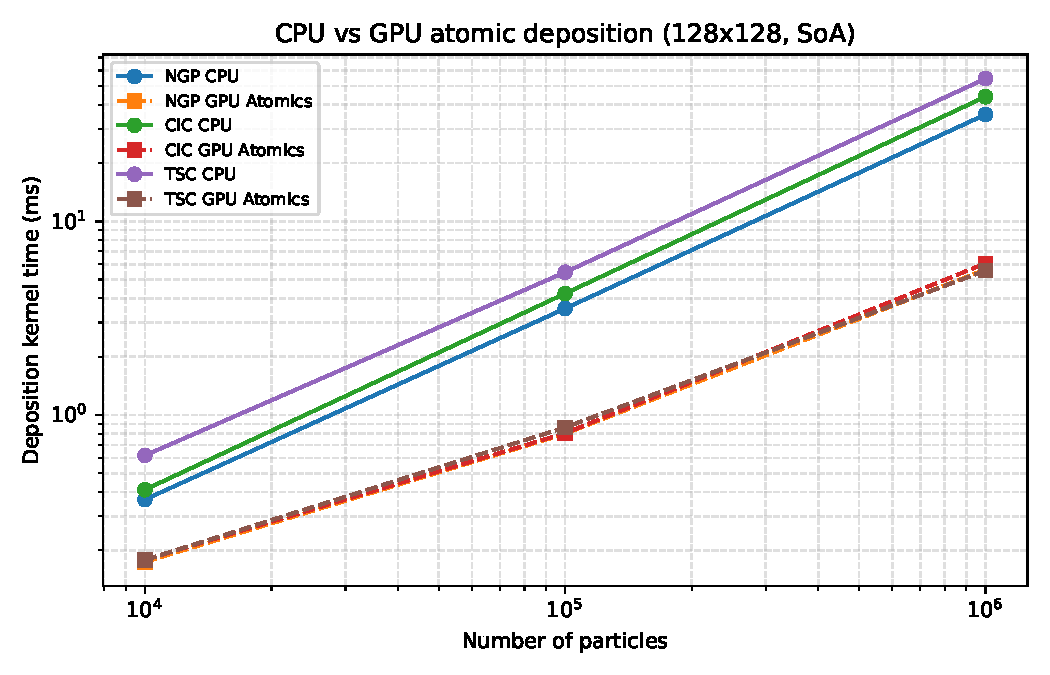
\includegraphics[width=\linewidth]{figures/fig8_gpu_runtime.pdf}
    \caption{CPU vs.\ GPU atomic deposition runtime ($128\times128$ grid, SoA, Tesla T4).}
    \label{fig:gpu_runtime}
\end{figure}

\begin{figure}[t]
    \centering
    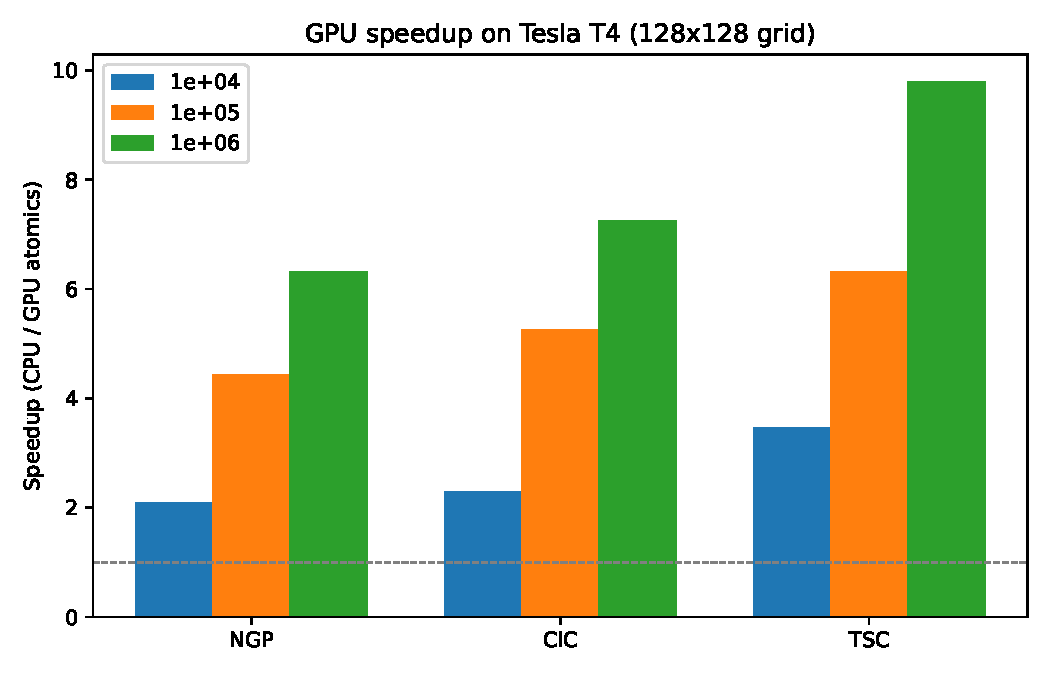
\includegraphics[width=\linewidth]{figures/fig9_gpu_speedup.pdf}
    \caption{GPU atomic speedup relative to T4-host CPU ($128\times128$ grid).}
    \label{fig:gpu_speedup}
\end{figure}

\begin{table}[t]
\centering
\small
\caption{CPU vs GPU atomic deposition on Tesla T4 ($N_p=10^5$, $128^2$ grid, SoA).}
\label{tab:gpu_summary}
\begin{tabular}{lrrr}
\toprule
Scheme & CPU (ms) & GPU (ms) & Speedup \\
\midrule
NGP & 3.55 & 0.80 & 4.4$\times$ \\
CIC & 4.24 & 0.81 & 5.3$\times$ \\
TSC & 5.46 & 0.86 & 6.3$\times$ \\
\bottomrule
\end{tabular}
\end{table}

\begin{table}[t]
\centering
\small
\caption{GPU atomic vs privatized CIC on Tesla T4 ($128^2$ grid, SoA).}
\label{tab:gpu_priv}
\begin{tabular}{lrrrr}
\toprule
$N_p$ & Atomics (ms) & Priv (ms) & Atomics speedup & Priv speedup \\
\midrule
1e+04 & 0.18 & 0.57 & 2.3$\times$ & 0.7$\times$ \\
1e+05 & 0.81 & 4.72 & 5.3$\times$ & 0.9$\times$ \\
1e+06 & 6.07 & 39.59 & 7.3$\times$ & 1.1$\times$ \\
\bottomrule
\end{tabular}
\end{table}


\subsection{Langmuir-Wave Validation}
All four schemes reproduce the same dominant oscillation frequency $\omega_{\mathrm{meas}} = 0.122$ within 5\% of one another, confirming scheme-independent linear physics in this test.
The ratio $\omega_{\mathrm{meas}}/\omega_{p,\mathrm{macro}} \approx 1.73$ is identical across NGP, CIC, TSC, and Esirkepov, indicating a systematic offset from the 1D cold-plasma estimate rather than scheme-dependent error.
TSC achieves the lowest spectral noise (0.26) while preserving the same measured frequency as CIC.
